%!TEX TS-program = xelatex

% Шаблон документа LaTeX создан в 2018 году
% Алексеем Подчезерцевым
% В качестве исходных использованы шаблоны
% 	Данилом Фёдоровых (danil@fedorovykh.ru) 
%		https://www.writelatex.com/coursera/latex/5.2.2
%	LaTeX-шаблон для русской кандидатской диссертации и её автореферата.
%		https://github.com/AndreyAkinshin/Russian-Phd-LaTeX-Dissertation-Template

\documentclass[a4paper,14pt]{article}


%%% Работа с русским языком
\usepackage[english,russian]{babel}   %% загружает пакет многоязыковой вёрстки
\usepackage{fontspec}      %% подготавливает загрузку шрифтов Open Type, True Type и др.
\defaultfontfeatures{Ligatures={TeX},Renderer=Basic}  %% свойства шрифтов по умолчанию
\setmainfont[Ligatures={TeX,Historic}]{Times New Roman} %% задаёт основной шрифт документа
\setsansfont{Comic Sans MS}                    %% задаёт шрифт без засечек
\setmonofont{Courier New}
\usepackage{indentfirst}
\frenchspacing

\renewcommand{\epsilon}{\ensuremath{\varepsilon}}
\renewcommand{\phi}{\ensuremath{\varphi}}
\renewcommand{\kappa}{\ensuremath{\varkappa}}
\renewcommand{\le}{\ensuremath{\leqslant}}
\renewcommand{\leq}{\ensuremath{\leqslant}}
\renewcommand{\ge}{\ensuremath{\geqslant}}
\renewcommand{\geq}{\ensuremath{\geqslant}}
\renewcommand{\emptyset}{\varnothing}

%%% Дополнительная работа с математикой
\usepackage{amsmath,amsfonts,amssymb,amsthm,mathtools} % AMS
\usepackage{icomma} % "Умная" запятая: $0,2$ --- число, $0, 2$ --- перечисление

%% Номера формул
%\mathtoolsset{showonlyrefs=true} % Показывать номера только у тех формул, на которые есть \eqref{} в тексте.
%\usepackage{leqno} % Нумерация формул слева	

%% Перенос знаков в формулах (по Львовскому)
\newcommand*{\hm}[1]{#1\nobreak\discretionary{}
	{\hbox{$\mathsurround=0pt #1$}}{}}

%%% Работа с картинками
\usepackage{graphicx}  % Для вставки рисунков
\graphicspath{{images/}}  % папки с картинками
\setlength\fboxsep{3pt} % Отступ рамки \fbox{} от рисунка
\setlength\fboxrule{1pt} % Толщина линий рамки \fbox{}
\usepackage{wrapfig} % Обтекание рисунков текстом

%%% Работа с таблицами
\usepackage{array,tabularx,tabulary,booktabs} % Дополнительная работа с таблицами
\usepackage{longtable}  % Длинные таблицы
\usepackage{multirow} % Слияние строк в таблице
\usepackage{float}% http://ctan.org/pkg/float

%%% Программирование
\usepackage{etoolbox} % логические операторы


%%% Страница
\usepackage{extsizes} % Возможность сделать 14-й шрифт
\usepackage{geometry} % Простой способ задавать поля
\geometry{top=20mm}
\geometry{bottom=20mm}
\geometry{left=20mm}
\geometry{right=10mm}
%
%\usepackage{fancyhdr} % Колонтитулы
% 	\pagestyle{fancy}
%\renewcommand{\headrulewidth}{0pt}  % Толщина линейки, отчеркивающей верхний колонтитул
% 	\lfoot{Нижний левый}
% 	\rfoot{Нижний правый}
% 	\rhead{Верхний правый}
% 	\chead{Верхний в центре}
% 	\lhead{Верхний левый}
%	\cfoot{Нижний в центре} % По умолчанию здесь номер страницы

\usepackage{setspace} % Интерлиньяж
\onehalfspacing % Интерлиньяж 1.5
%\doublespacing % Интерлиньяж 2
%\singlespacing % Интерлиньяж 1

\usepackage{lastpage} % Узнать, сколько всего страниц в документе.

\usepackage{soul} % Модификаторы начертания

\usepackage{hyperref}
\usepackage[usenames,dvipsnames,svgnames,table,rgb]{xcolor}
\hypersetup{				% Гиперссылки
	unicode=true,           % русские буквы в раздела PDF
	pdftitle={Заголовок},   % Заголовок
	pdfauthor={Автор},      % Автор
	pdfsubject={Тема},      % Тема
	pdfcreator={Создатель}, % Создатель
	pdfproducer={Производитель}, % Производитель
	pdfkeywords={keyword1} {key2} {key3}, % Ключевые слова
	colorlinks=true,       	% false: ссылки в рамках; true: цветные ссылки
	linkcolor=black,          % внутренние ссылки
	citecolor=black,        % на библиографию
	filecolor=magenta,      % на файлы
	urlcolor=black           % на URL
}
\makeatletter 
\def\@biblabel#1{#1. } 
\makeatother
\usepackage{cite} % Работа с библиографией
%\usepackage[superscript]{cite} % Ссылки в верхних индексах
%\usepackage[nocompress]{cite} % 
\usepackage{csquotes} % Еще инструменты для ссылок

\usepackage{multicol} % Несколько колонок

\usepackage{tikz} % Работа с графикой
\usepackage{pgfplots}
\usepackage{pgfplotstable}

% ГОСТ заголовки
\usepackage[font=small]{caption}
%\captionsetup[table]{justification=centering, labelsep = newline} % Таблицы по правобу краю
%\captionsetup[figure]{justification=centering} % Картинки по центру


\newcommand{\tablecaption}[1]{\addtocounter{table}{1}\small \begin{flushright}\tablename \ \thetable\end{flushright}%	
\begin{center}#1\end{center}}

\newcommand{\imref}[1]{рис.~\ref{#1}}

\usepackage{multirow}
\usepackage{spreadtab}
\newcolumntype{K}[1]{@{}>{\centering\arraybackslash}p{#1cm}@{}}


\usepackage{xparse}
\usepackage{fancyvrb}

\RecustomVerbatimCommand{\VerbatimInput}{VerbatimInput}
{
	fontsize=\footnotesize    
}

\usepackage{tocloft}
\renewcommand{\cftsecleader}{\cftdotfill{\cftdotsep}}
\begin{document} % конец преамбулы, начало документа
	\begin{titlepage}
	\begin{center}
 		ФЕДЕРАЛЬНОЕ  ГОСУДАРСТВЕННОЕ АВТОНОМНОЕ \\
		ОБРАЗОВАТЕЛЬНОЕ УЧРЕЖДЕНИЕ ВЫСШЕГО ОБРАЗОВАНИЯ\\
		«НАЦИОНАЛЬНЫЙ ИССЛЕДОВАТЕЛЬСКИЙ УНИВЕРСИТЕТ\\
		«ВЫСШАЯ ШКОЛА ЭКОНОМИКИ»
	\end{center}
	
	\begin{center}
		\textbf{Московский институт электроники и математики}
		
		\textbf{им. А.Н.Тихонова НИУ ВШЭ}
		
		\vspace{2ex}
		
		\textbf{Департамент компьютерной инженерии}
	\end{center}
	\vspace{1ex}	
	
	\begin{center}
		Курс «Системное проектирование цифровых устройств»
	\end{center}	
	
	
	\begin{center}
	\textbf{ОТЧЕТ\\
		ПО ЛАБОРАТОРНОЙ РАБОТЕ №5
	}
	\end{center}	

	\begin{center}
		Тема работы: «Обработка звука на ПЛИС»
	\end{center}

	\vspace{2ex}

	\begin{flushright}
		\textbf{Выполнили:}
		
		\vspace{2ex}
		
		Студенты группы БИВ174
		
		Бригада №5
		
		\vspace{2ex}
		
		Подчезерцев Алексей Евгеньевич
		
		Солодянкин Андрей Александрович
		\vspace{2ex}
		
		\textbf{Принял:}
		
		асс. МИЭМ НИУ ВШЭ
		
		Американов А.А.
		
	\end{flushright}

	\vfill
	\begin{center}
		Москва \the\year \, г.
	\end{center}
	
\end{titlepage}
\addtocounter{page}{1}
	\tableofcontents
	\pagebreak
	\section{Задание}
	
	\begin{enumerate}
		\item В соответствии с мануалом Altera\_QurtusII\_SignalTap\_manual.pdf создать простой проект, где на светодиоды подаются комбинации нажатия на кнопки по принципу дешифратора.
		
		\item Скомпилировать проект и выполнить прототипирование, убедиться в корректности работы проекта.
		
		\item Включить Quartus II TalkBack Feature.
		
		\item Запустить SignalTap II и в соответствии с мануалом настроить отслеживание нажатия следующей комбинации кнопок = ваш вариан\% 4 +1.
		
		\item Привязать тактовый сигнал.
		
		\item Выполнить компиляцию проекта. Запрограммировать плату. Отследить событие нажатия комбинации кнопок. Привести результаты в отчете.
		
		\item Отследить события прихода фронтов сигналов для комбинации кнопок = (ваш вариант+1)\% 4 +1. Продемонстрировать отличия от отслеживания события по уровню.
		
		\item Добавить собственные условия для срабатывания событий в режиме Advanced.
			
		\item Настроить множественное отслеживание событий используя Sample Depth and Buffer Acquisition Modes.
		
		\item Проиллюстрировать на своем проекте использование Synthesis Keep Directive и необходимость ее использования.
		
		\item Оформить отчет.
		
		\item Используя проект из Практической работы 1, сделать его копию.
		Не добавляя дополнительную периферию выполнить отслеживание состояний регистров в регистровом файле.
		С использованием SignalTap II продемонстрировать корректность выполнение программ 00\_counter/, 01\_fibonacci/ и 02\_sqrt/.
		
		\item Перейти в ветку проекта schoolMIPS 03\_pipeline\_irq: https://github.com/MIPSfpga/schoolMIPS/tree/04\_pipeline\_irq.
		Скачать новую версию процессора и выполнить на вашей плате (или DE10-Lite) программы https://github.com/MIPSfpga/schoolMIPS/tree/04\_pipeline\_irq/program, в программах начиная с 4-й сделать подробные комментарии. Объяснить, чем эта версия schoolMIPS отличается от базовой.
		
		\item Перейти в ветку проекта schoolMIPS 05\_pipeline\_ahb: https://github.com/MIPSfpga/schoolMIPS/tree/05\_pipeline\_ahb.
		Скачать новую версию процессора и выполнить на вашей плате (или DE10-Lite) программы https://github.com/MIPSfpga/schoolMIPS/tree/05\_pipeline\_ahb/program, в программах начиная с 4-й сделать подробные комментарии. Объяснить, чем эта версия schoolMIPS отличается от базовой.
		
	\end{enumerate}

	%{\small \VerbatimInput{../03_syn_pow_5_single_cycle_always/pow_5_single_cycle_always.v}}
	
	\section{Выполнение работы}
	
	Был создан проект, который представляет из себя простейший дешифратор.
	Код дешифратора:
	
	{\small \VerbatimInput{../first_part/de0_cv/project/keys.v}}
	
	Проект скомпилировался, его RTL представление (рис. \ref{fig:rtl}) и вейвформа (рис. \ref{fig:wvf}).
	
	\begin{figure}[H]
		\centering
		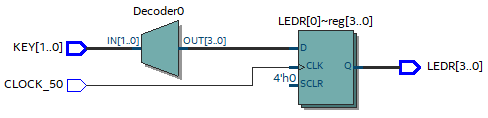
\includegraphics[width=0.6\linewidth]{images/RTL}
		\caption{RTL представление проекта}
		\label{fig:rtl}
	\end{figure}

	\begin{figure}[H]
		\centering
		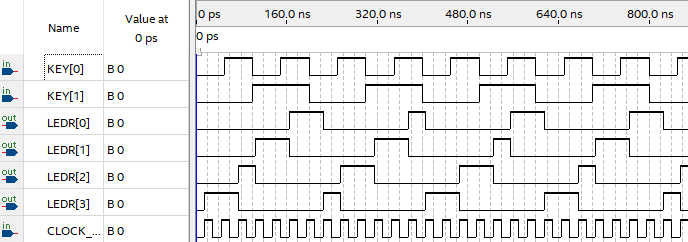
\includegraphics[width=0.6\linewidth]{images/WVF}
		\caption{Моделирование проекта}
		\label{fig:wvf}
	\end{figure}
	
	Тактовый сигнал привязан.
	
	Отслеживание нужной комбинации проводилось при помощи $SignalTap$, таблица $setup$ представлена на рис. \ref{fig:setupkey1}.
	
	\begin{figure}[H]
		\centering
		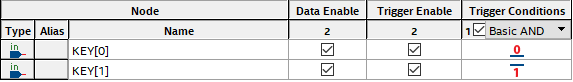
\includegraphics[width=0.7\linewidth]{images/setup_key_1}
		\caption{Таблица setup для отслеживания нужной комбинации}
		\label{fig:setupkey1}
	\end{figure}

	Отслеживание приходов фронтов проводилось в режиме $advanced$.
	Т. к. одновременный приход двух фронтов на частоте 50 МГц почти невозможен, будем отслеживать интересующую нас комбинацию по последнему фронту, т. е. один из ключей уже должен быть в нужном положении.
	Схема в $advanced$ режиме представлена на рис. \ref{fig:advancedscheme}.

	\begin{figure}[H]
		\centering
		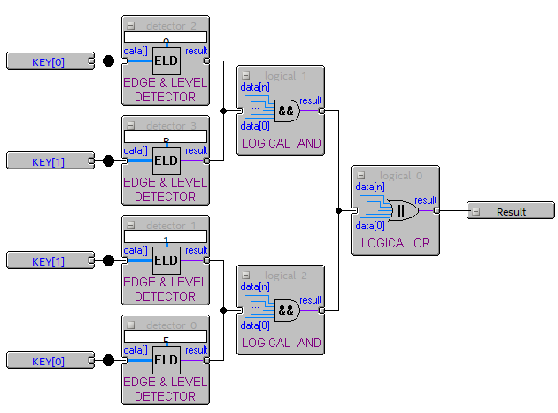
\includegraphics[width=0.7\linewidth]{images/advanced_scheme}
		\caption{$advanced$ схема для отслеживания фронтов}
		\label{fig:advancedscheme}
	\end{figure}

	Если зажать нужную комбинацию и запустить отслеживание комбинации по фронту, то комбинация не будет замечена.
	Если запустить отслеживание по уровню, то комбинация будет обнаружена.
	
	Было настроено множественное отслеживание событий используя $Sample Depth$ и $Buffer Acquisition Modes$.

	$Synthesis Keep Directive$ необходима для того, чтобы квартус при компиляции не убирал необходимые для анализа сигналы.
	На рис. \ref{fig:rtl1} схема с RTL представление с $Synthesis Keep Directiv$, а на рис. \ref{fig:rtl2} схема без RTL представление с $Synthesis Keep Directiv$.
	Можно заметить, что на рис. \ref{fig:rtl2} пропал сигнал $w1$.
	
	\begin{figure}[H]
		\centering
		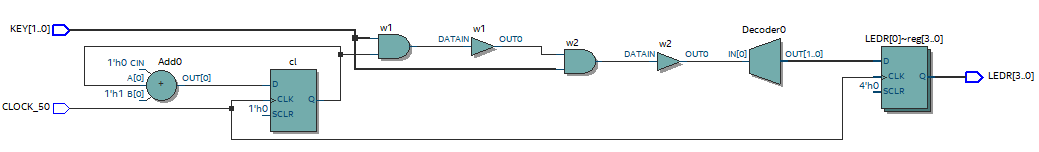
\includegraphics[width=0.7\linewidth]{images/rtl_1}
		\caption{RTL представление с $Synthesis Keep Directive$}
		\label{fig:rtl1}
	\end{figure}
	
	
	\begin{figure}[H]
		\centering
		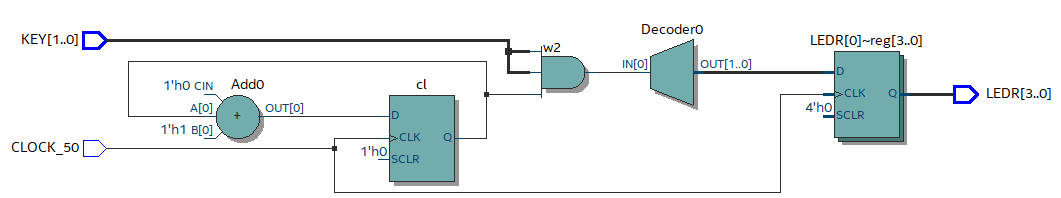
\includegraphics[width=0.7\linewidth]{images/rtl_2}
		\caption{RTL представление без $Synthesis Keep Directive$}
		\label{fig:rtl2}
	\end{figure}	
	
	\section{Самостоятельная работа}
	
	\subsection{Настройка SignalTap для 1 версии процессора}
	
	В таблицу $setup$ были перенесены первые 16 регистров процессора, а также кнопка $KEY_2$ по убывающему фронту которой будет начинаться запись из выбранных регистров.
	
	\begin{figure}[H]
		\centering
		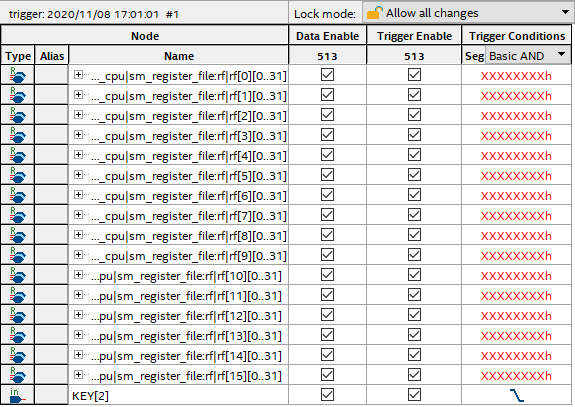
\includegraphics[width=0.7\linewidth]{images/view_registers}
		\caption{Таблица $setup$ для отслеживания состояния регистров}
		\label{fig:viewregisters}
	\end{figure}
	
	

	\subsection{Моделирование программ на процессоре \\ из ветки 04\_pipeline\_irq}
	
	Было произведено моделирование программ  00\_counter, 01\_fibonacci, 02\_sqrt, 03\_ram, все по-прежнему работают, но никаких изменений в логах или вейвформах нет.
	
	Данный процессор отличается о базового прежде всего тем, что данный процессор является конвейерным.
	Также в этой версии процессора реализованы прерывания для обработки исключений.
	Данной задачей занимается сопроцессор $sm\_cpz$.
	%04_04_irq_timer
	%04_05_exc_ri
	%04_06_hz_forward
	%04_07_hz_stall
	%04_08_hz_branch
	\subsubsection{Моделирование программы 04\_irq\_timer}
	
	В соответствии с вариантом была смоделирована программа 04\_irq\_timer.
	В данной программе демонстрируется возможный функционал обработки исключений.
	Ее ассемблерный код:
	
	{\small \VerbatimInput{../branch_04/04_pipeline_irq/04_irq_timer/main.S}}
	
	Ниже приведена часть логов из выполнения программы:
	
	{\small \VerbatimInput{./logs/04_04_irq_timer.txt}}
	
	Вейвформа при моделировании программы (рис. \ref{fig:0404wvf}).
	
	\begin{figure}[H]
		\centering
		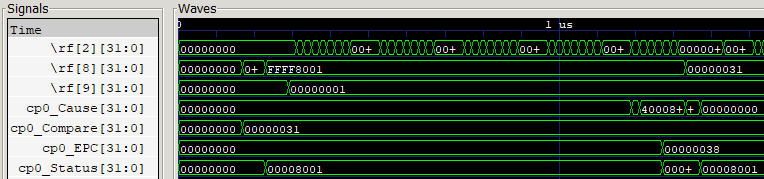
\includegraphics[width=0.95\linewidth]{images/04_04_wvf}
		\caption{Вейвформа для  04\_irq\_timer}
		\label{fig:0404wvf}
	\end{figure}

	\subsubsection{Моделирование программы 05\_exc\_ri}
	
	В соответствии с вариантом была смоделирована программа  05\_exc\_ri.
	В данной программе демонстрируется возможный функционал обработки исключений.
	Ее ассемблерный код:
	
	{\small \VerbatimInput{../branch_04/04_pipeline_irq/05_exc_ri/main.S}}
	
	Ниже приведена часть логов из выполнения программы:
	
	{\small \VerbatimInput{./logs/04_05_exc_ri.txt}}
	
	Вейвформа при моделировании программы (рис. \ref{fig:0405wvf}).
	
	\begin{figure}[H]
		\centering
		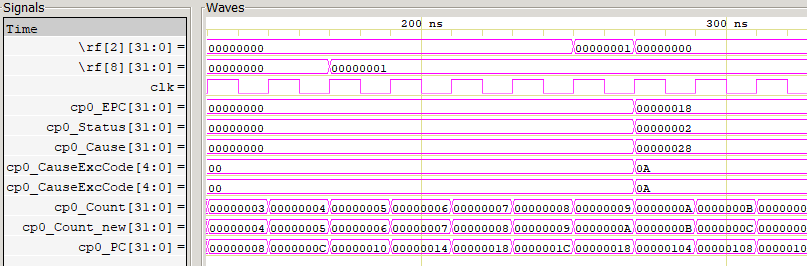
\includegraphics[width=0.95\linewidth]{images/04_05_wvf}
		\caption{Вейвформа для  05\_exc\_ri}
		\label{fig:0405wvf}
	\end{figure}
		
		
	\subsubsection{Моделирование программы 06\_hz\_forward}
	
	В соответствии с вариантом была смоделирована программа 06\_hz\_forward.
	В данной программе проверяется работа конвейера при доступе к данным.
	Ее ассемблерный код:
	
	{\small \VerbatimInput{../branch_04/04_pipeline_irq/06_hz_forward/main.S}}
	
	Ниже приведена часть логов из выполнения программы:
	
	{\small \VerbatimInput{./logs/04_06_hz_forward.txt}}
	
	Вейвформа при моделировании программы (рис. \ref{fig:0406wvf}).
	
	\begin{figure}[H]
		\centering
		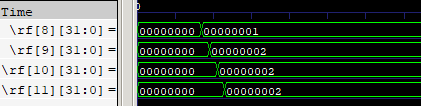
\includegraphics[width=0.7\linewidth]{images/04_06_wvf}
		\caption{Вейвформа для  06\_hz\_forward}
		\label{fig:0406wvf}
	\end{figure}

	\subsubsection{Моделирование программы 07\_hz\_stall}
	
	В соответствии с вариантом была смоделирована программа  07\_hz\_stall.
	В данной программе продемонстрирована возможность тупиковой ситуации.
	Ее ассемблерный код:
	
	{\small \VerbatimInput{../branch_04/04_pipeline_irq/07_hz_stall/main.S}}
	
	Ниже приведена часть логов из выполнения программы:
	
	{\small \VerbatimInput{./logs/04_07_hz_stall.txt}}
	
	Вейвформа при моделировании программы (рис. \ref{fig:0407wvf}).
	
	\begin{figure}[H]
		\centering
		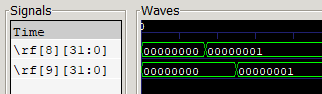
\includegraphics[width=0.6\linewidth]{images/04_07_wvf}
		\caption{Вейвформа для  07\_hz\_stall}
		\label{fig:0407wvf}
	\end{figure}
	
	
	\subsubsection{Моделирование программы 08\_hz\_branch}
	
	В соответствии с вариантом была смоделирована программа 08\_hz\_branch.
	В данной программе проверяется работа конвейера в различных ситуациях ветвления.
	Ее ассемблерный код:
	
	{\small \VerbatimInput{../branch_04/04_pipeline_irq/08_hz_branch/main.S}}
	
	Ниже приведена часть логов из выполнения программы:
	
	{\small \VerbatimInput{./logs/04_08_hz_branch.txt}}
	
	Вейвформа при моделировании программы (рис. \ref{fig:0408wvf}).
	
	\begin{figure}[H]
		\centering
		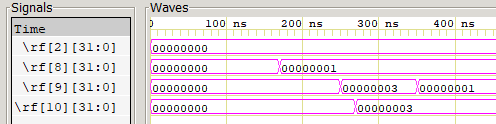
\includegraphics[width=0.95\linewidth]{images/04_08_wvf}
		\caption{Вейвформа для  08\_hz\_branch}
		\label{fig:0408wvf}
	\end{figure}
	
	\subsection{Моделирование программ на процессоре \\ из ветки 05\_pipeline\_ahb}
	
	Программы 00 -- 07 по прежнему работают. Изменений в вейвформах и логах нет.
	В данную версию добавлена Advanced High-performance Bus (AHB) Lite версии,
	которая позволяет взаимодействовать двум и более устройствам в режиме master~--~slaves.
	
	\subsubsection{Моделирование программы 09\_ahb\_mem}
	
	В данной программе проверяется работа памяти путем постоянного чтения и записи по разным адресам.
	Ее ассемблерный код:
	
	{\small \VerbatimInput{../branch_05/05_pipeline_ahb/09_ahb_mem/main.S}}
	
	Ниже приведена часть логов из выполнения программы:
	
	{\small \VerbatimInput{./logs/05_09_ahb_mem.txt}}
	
	Вейвформа при моделировании программы (рис. \ref{fig:05_09_wvf}).
	
	\begin{figure}[H]
		\centering
		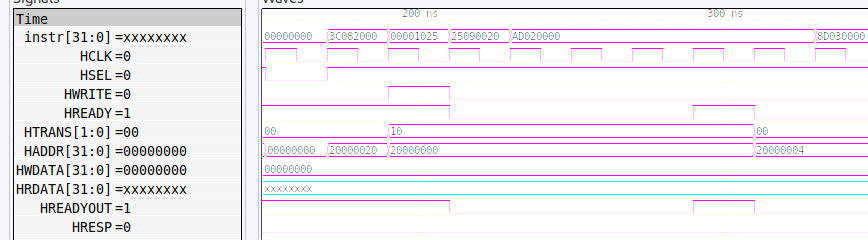
\includegraphics[width=\linewidth]{images/05_09_wvf}
		\caption{Вейвформа для  09\_ahb\_mem}
		\label{fig:05_09_wvf}
	\end{figure}

	\subsubsection{Моделирование программы 10\_ahb\_gpio}

	В данной программе проверяется работа GPIO путем постоянного чтения и записи по разным адресам.
	Ее C код:
	
	{\small \VerbatimInput{../branch_05/05_pipeline_ahb/10_ahb_gpio/main.c}}
	
	Ниже приведена часть логов из выполнения программы:
	
	{\small \VerbatimInput{./logs/05_10_ahb_gpio.txt}}
	
	Вейвформа при моделировании программы (рис. \ref{fig:05_10_wvf}).
	
	\begin{figure}[H]
		\centering
		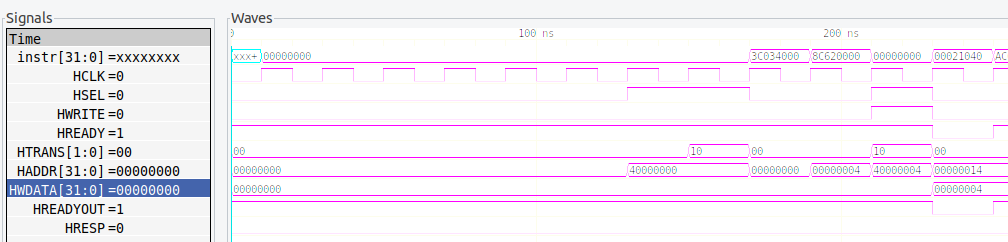
\includegraphics[width=\linewidth]{images/05_10_wvf}
		\caption{Вейвформа для 10\_ahb\_gpio}
		\label{fig:05_10_wvf}
	\end{figure}

	\section{Выводы по работе}
	
	В ходе работы получен опыт в написании кода на ассемблере MIPS.
	Был получен опыт чтения машинного кода.
	Была исследован функционал SignalTap в программе Qurtus.
	Были исследованы Advanced, Sample Depth и Buffer Acquisition Modes в SignalTap.
	Был протестирован функционал Synthesis Keep Directive.
	Было произведено моделирование в программе Icarus Verilog.
	Итоговый проект был собран и загружен на плату.

	
	\newpage 
	\renewcommand{\refname}{{\normalsize Список использованных источников}} 
	\centering 
	\begin{thebibliography}{9} 
		\addcontentsline{toc}{section}{\refname} 
		\bibitem{Harris} Хэррис Д. М., Хэррис С. Л. Цифровая схемотехника и архитектура компьютера. – 2015.
	\end{thebibliography}
	
\end{document} % конец документа
